\subsection{Exploration du dataset}

Le fichier d'entraînement train\_submissions.csv proposé pour cette compétition kaggle est un fichier csv de 3 colonnes Usage, Text, Label et 190599 lignes avec 389 labels cibles. Parmi ces 190599 lignes, 500 d'entre elles ne possèdent pas de label. 

On peut noter que les labels sont déséquilibrés, comme le montre la figure suivante :

\begin{figure}[h!]
    \centering
    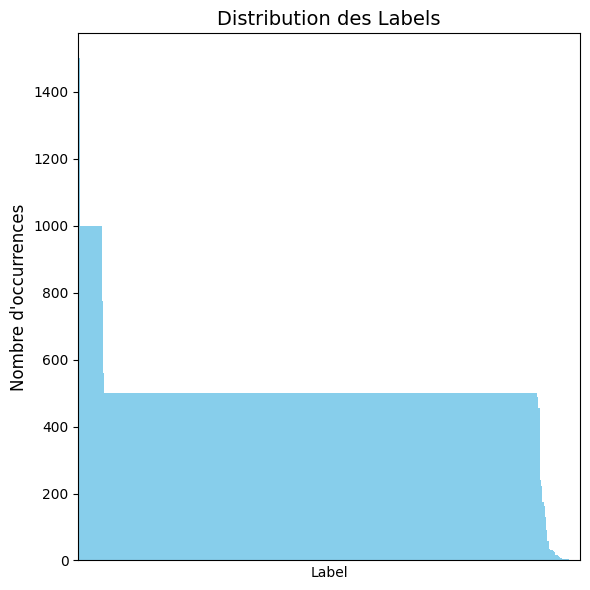
\includegraphics[width=0.5\textwidth, height=7cm]{img/unbalance.png}
    \caption{Distribution déséquilibrée des labels dans le dataset}
    \label{fig:unbalance}
\end{figure}

Nous avons essayé plusieurs techniques de downsampling et d'oversampling pour palier au déséquilibre des données, notamment en essayant d'enrichir les labels avec le moins de données disponibles grâce à des LLMs. Néanmoins cette approche n'a pas donné de bon résultats car cela retirait une partie des biais inhérents au dataset. Nous avons donc fait le choix de downsampler les labels ayant plus de 500 labels en choisissant 500 lignes aléatoirement parmi ces labels.

Il est à noté que le dataset comprenait de nombreuses langues régionales très peu parlées donc males prises en charge par de nombreux modèles pré-entrainé. De plus, pour ces langues la quantité de données pour l'entrainement était assez faible puisque plus de 50\% des textes ne comportaient pas plus de 16 mots. 

\begin{figure}[h!]
    \centering
    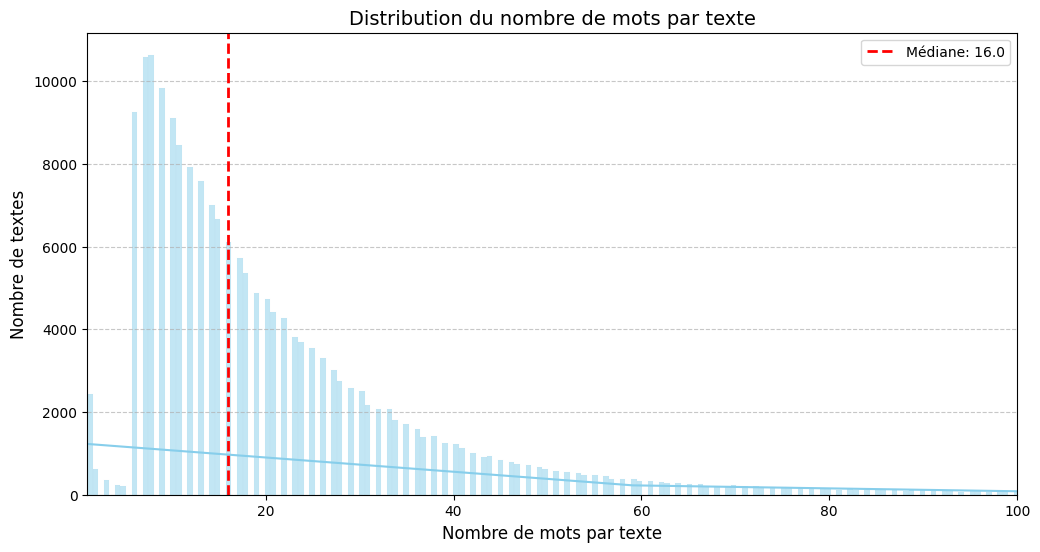
\includegraphics[width=0.5\textwidth, height=7cm]{img/word_count.png}
    \caption{Nombre de mots par texte.}
    \label{fig:unbalance}
\end{figure}

Enfin nous pouvons également souligné la présence de nombreuses langues très répandues telles que l'anglais, l'espagnol ou encore le français qui représentait parfois la totalité de certains textes pourtant labellisé dans une autre langue. C'est pourquoi lors de nos différentes tentatives le recall obtenu sur ces différentes langues s'avérait plus faible comparativement à des langues moins usitées.

\subsection{Preprocessing}
Les données sont parfois bruitées : certaines contiennent du code html, des adresses mails ou encore des emojis. En outre, certaines données contiennent beaucoup de mots en anglais (ou autre langue très parlée), voire sont mal classifiées : cela s'explique notamment par le fait que les données proviennent de site tels que twitter, où beaucoup d'utilisateurs utilisent l'anglais par soucis de compréhension. Le preprocessing a donc été notamment tourné vers l'identification et l'élimination du bruit. Nous avons prévu deux preprocessing : suppression des charactères non pertinents (emojis, balises html, ...) et suppression des mots en anglais, français et espagnol lorsqu'ils sont minoritaires dans la phrase.

Pour la suppression des caractères non pertinents, nous avons utilisé des règles regex. Cependant, l'impact sur la qualité des prédictions n'a pas été très important : cela pourrait s'expliquer par la suppression de biais présents dans certaines langues, biais qui proviennent du scrapping de sources similaires et qui créent des similarités intra-classes ne provenant pas du langage. Par exemple, on pourrait imaginer que les données disponibles pour une langue ont été intégralement prises d'un compte Twitter/X, ce qui pourrait créer un biais sur l'utilisation de certains emojis.

Pour la suppression des mots en anglais, français, espagnol, nous avons utilisé des bases de données de mots provenant d'un github (\cite{hermitdave2018frequency}). Nous avons utilisé un seuil : si les mots repérés sont minoritaires dans la phrase (moins de 50\% de la phrase), nous avons considéré que ces mots étaient empruntés à l'anglais, au français ou à l'espagnol, et avons retiré ces mots des phrases. Cette démarche n'a pas été très concluante : cela s'explique notamment par la présence de dialectes (par exemple, l'argentin) qui partagent de nombreux mots avec d'autres langues.

Finalement, nous avons choisi d'utiliser le dataset tel quel, et de concentrer nos efforts sur les modèles utilisés.
\subsection{TF-IDF}

TF-IDF est une méthode statistique utilisée pour évaluer l'importance d'un mot dans un document par rapport à une collection de documents. Elle combine deux métriques : la fréquence du terme (TF) et la fréquence inverse du document (IDF). La fréquence du terme mesure combien de fois un mot apparaît dans un document, tandis que l'IDF diminue l'importance des mots qui apparaissent fréquemment dans tous les documents.

Pour notre utilisation, TF-IDF nous permet de créer des vecteurs de représentation à partir des textes, puis d'entraîner un classifieur pour évaluer la langue du texte. Dans notre cas, nous avons utilisé un classifieur SVM car c'est celui qui, théoriquement et expérimentalement, donne les meilleurs résultats (voir \cite{baldwin2010language}).

Cette approche nous a donné des résultats assez satisfaisants mais pas suffisants pour notre cas d'utilisation et s'est laissé largement dépasser par les autres approches, certainement car elle ne prend pas en compte les relations entre les mots et les contextes dans lesquels ils apparaissent.

\subsection{FastText}

FastText est une bibliothèque développée par Facebook \cite{joulin2017bag} pour la représentation de mots et l'apprentissage de classificateurs de texte. Comme vu en cours, elle repose sur des modèles de type n-grammes pour capturer des informations sur les sous-mots, ce qui permet de mieux gérer les mots rares et les fautes d'orthographe.

FastText est particulièrement efficace pour l'identification de langue car il peut capturer des caractéristiques spécifiques à chaque langue au niveau des sous-mots. Il a donné de très bons résultats dans notre étude, avec des scores similaires voire supérieurs aux modèles de langage neuronaux (voir ci-dessous), mais avec des temps d'entraînement et d'inférence presque instantanés en comparaison.

Pour son entraînement, nous avons dans un premier temps pris les hyperparamètres donnés dans l'article GlotLID \cite{Kargaran_2023}, un article présentant un modèle classifiant plus de 1800 langues, puis nous avons fait une recherche d'hyperparamètres aux alentours de ces derniers. 

\begin{table}[h]
    \centering
    \small
    \begin{tabular}{lcc}
        \hline
        \textbf{Argument} & \textbf{Description} & \textbf{Valeur} \\
        \hline
        -minCount & Occurrences min mot & 1000 \\
        -minCountLabel & Occurrences min label & 0 \\
        -wordNgrams & Max n-grammes mots & 1 \\
        -bucket & Nb de buckets & $10^6$ \\
        -minn & Min. n-gram caractères & 1 \\
        -maxn & Max. n-gram caractères & 5 \\
        -loss & Perte & softmax \\
        -dim & Taille vecteurs & 256 \\
        -epoch & Nombre d'époques & 9 \\
        -lr & Taux apprentissage & 1.5 \\
        \hline
    \end{tabular}
    \caption{Hyperparamètres d'entraînement du modèle FastText}
    \label{tab:glotlid-m-hyperparams}
\end{table}

\subsection{mBERT}

mBERT (Multilingual BERT) est la version multilingue du modèle BERT \cite{devlin2019bert}, qui est un modèle de langage basé sur des transformers, possédant 179M de paramètres. Sa particularité est qu'il est pré-entraîné sur la tâche de Masked Language Model, sur un vaste corpus de textes dans 104 langues, ce qui lui permet de comprendre et de générer des représentations contextuelles pour des textes dans différentes langues.

Ce modèle fut notre première approche de langage neuronal pour ce projet.  Nous avons de même utilisé le tokenizer correspondant à mBERT, comprenant tous les caractères de notre corpus, et nous n'avons pas mis de limite de taille pour le nombre de tokens. Nous avons d'abord essayé une méthode de transfert (transfer learning) pour adapter mBERT à notre tâche, mais cela s'est avéré insuffisant et il a finalement fallu ajuster les poids du modèle (fine-tuning) pour obtenir des résultats satisfaisants sur 10 epochs, en utilisant 85\% du dataset fourni en train, et une dernière epoch en utilisant la totalité du corpus, pour utiliser le plein potentiel de nos données. L'inconvénient de cette méthode est qu'elle est très lourde en calculs (plusieurs heures d'entraînement).

Finalement, mBERT a donné des résultats satisfaisants mais s'est logiquement laissé dépasser par XLM-RoBERTa (voir ci-dessous), qui possède en particulier plus de paramètres.

\subsection{XLM-RoBERTa}

XLM-RoBERTa \cite{conneau2020unsupervised} est une variante optimisée de BERT \cite{devlin2019bert} qui utilise un processus d'entraînement plus robuste et une plus grande quantité de données sur 100 langues. Nous avons utilisé le modèle base à 279M de paramètres. Les améliorations incluent l'entraînement sur des lots de données plus grands, l'utilisation de plus de données d'entraînement, et l'optimisation des hyperparamètres. C'est donc très logiquement que nos résultats suivent l'amélioration promise par les chercheurs à son origine et qu'il surpasse mBERT.

Notre utilisation reprend la même logique que pour mBERT avec une nette amélioration des performances, mais avec un coût en temps d'entraînement et d'inférence plus élevé. Pour palier à cela, nous avons décidé de restreindre chaque phrase à 128 tokens, avec un padding si la phrase contient moins de 128 tokens, et un troncage si elle en contient plus. Cela a drastiquement réduit le temps d'entraînement. Nous avons également utilisé un taux d'apprentissage de 2e-5, un batch size de 64, et un nombre d'époques de 10. On a de plus utilisé le tokenizer de XLM-RoBERTa.

\subsection{Combinaison FastText et XLM-RoBERTa}

Il nous est naturellement venu l'envie de combiner nos modèles portant sur des approches différentes pour tenter de profiter des avantages de chaques approches, pour améliorer les performances de notre solution. La combinaison qui nous a donné les meilleurs résultats après divers essais est la suivante : si l'inférence avec FastText donne une prédiction avec une probabilité supérieure à 0.99\%, on la garde ; sinon, on utilise XLM-RoBERTa pour donner une prédiction. Nous avons fait une étude de sensibilité sur le seuil de probabilité de FastText, et 0.99\% est le seuil qui nous a donné les meilleurs résultats, et, en effet, les prédictions au dessus de ce seuil ont une accuracy de 99\% sur le val.